\section{Experiments and results}

All videos were preprocessed by
separating the two streams into different files (replacing the small embedded view with black pixels),
resampling to 15 \ac{FPS} and $320 \times 180$ pixels,
and reencoding using \ac{HEVC}.
To avoid geometric distortions while maximizing the \ac{FOV} and resolution, videos were cropped horizontally by removing 5\,\% of the columns from each side, and padded vertically so frames were square.
Snippets were resized as imposed by the corresponding architecture to $224 \times 224$ for \acp{SFCNN} and  $112 \times 112$ for \acp{STCNN}.
For realism, six video streams in which the patient was completely outside of the \ac{FOV} were discarded for training but used for evaluation.
Recorded audio signals were discarded.

Experiments were implemented in PyTorch 1.7.0.
We used a stratified 10-fold cross-validation, generated to ensure the total duration of the videos and ratio of \acp{FOS} to \acp{FBTCS} were similar across folds.
Both views from the same video were assigned to the same fold, but videos from the same patient were not.
This is because individual patients can present with both \acp{FOS} or \acp{FBTCS}, so data leakage at the patient level is not a concern.
We minimized the weighted binary cross-entropy loss to overcome dataset imbalance, using the AdamW optimizer \cite{loshchilov_decoupled_2019}.
The code is available at \myhref{https://github.com/fepegar/gestures-miccai-2021}.

For each fold, evaluation is performed using the model from the epoch with the lowest validation loss.
At inference time, the network predicts probabilities for both video streams of a seizure, and these predictions are averaged.
The final binary prediction is the consensus probability thresholded at 0.5.
We analyzed differences in model performance using a one-tailed Mann-Whitney $U$ test (as metrics were not normally distributed) with a significance threshold of $\alpha = 0.05$, and Bonferroni correction for each set of $e$ experiments: $\alpha\st{Bonf} = \frac{\alpha}{e (e - 1)}$.


\subsection{Evaluation of feature extractors for snippets}
\label{sec:exp_feat}

Despite recent advances in \acp{STCNN} for \ac{HAR}, these architectures do not always outperform \acp{SFCNN} pre-trained on large generic datasets \cite{hutchinson_accuracy_2020}.
We assessed the ability of different feature extractors to model semiologies by training a classifier for snippet-level classification (\cref{sec:snippet-level}).

\begin{table}
  \setlength{\tabcolsep}{3pt}
  \centering
  \caption[Performance of the feature extractors]{
    Performance of the feature extractors.
    The number of parameters is shown in millions.
    AUC is the area under the precision-recall curve.
    Accuracy is computed for \acp{FBTCS} and \acp{FOS}, while $F_1$-score and AUC only for \acp{FBTCS}, represented by an asterisk (*).
    Metrics are expressed as `median (interquartile range)'.
  }
  \label{tab:models}
  \begin{tabular}{l*5c}
    \toprule
    \textbf{Model (frames)} & \textbf{Parameters} & \textbf{Features} & \textbf{Accuracy} & $\bm{F_1}$\textbf{-score}* & \textbf{AUC}* \\
    \midrule
    Wide R2D-50-2 (1)       &              66.8 M &              2048 &       80.3 (33.2) &                67.4 (30.2) &   75.7 (38.4) \\
    R2D-34 (1)              &              21.2 M &               512 &       89.7 (27.7) &                73.9 (23.6) &   84.3 (28.7) \\
    R(2+1)D-34 (8)          &              63.5 M &               512 &       93.9 (18.3) &                81.6 (16.9) &   93.7 (13.4) \\
    R(2+1)D-34 (32)         &              63.5 M &               512 &       96.9 (12.9) &                84.7 (13.4) &   94.7 (11.9) \\
    \bottomrule
  \end{tabular}
\end{table}

We used two pre-trained versions of the \ac{STCNN} R(2+1)D-34 \cite{ghadiyaram_large-scale_2019} that take as inputs 8 frames ($\approx \SI{0.5}{s}$) or 32 frames ($\approx \SI{2.1}{s}$).
Models were trained using weakly supervised learning on over 65 million Instagram videos and fully supervised learning on over 250,000 YouTube videos of human actions.
We selected two pre-trained \acp{SFCNN} with 34 (R2D-34) and 50 (Wide R2D-50-2) layers, trained on ImageNet \cite{zagoruyko_wide_2017}.
The \acp{SFCNN} were chosen so the numbers of layers (34) and parameters ($\approx 65$ million) were similar to the \acp{STCNN}.

To ensure that all features datasets have the same number of training instances, we divided each video into segments of 32 frames.
Then, we use the models to extract features from snippets of the required length (8, 32, or 1) such that all snippets are centered in the segments.
The datasets of extracted feature vectors are publicly available \cite{perez-garcia_data_2021}.
We trained a fully-connected layer for 400 epochs on each feature set, treating views from the same video independently.
We used an initial learning rate $10 ^ {-3}$ and mini-batches of 1024 feature vectors.
We minimized a weighted binary cross-entropy loss, where the weight for \acp{FBTCS} was computed as the ratio of \ac{FOS} frames to \ac{FBTCS} frames.

For evaluation, a sliding window was used to infer probabilities for all snippets.
\acp{STCNN} performance was significantly better than \acp{SFCNN} ($p < 10 ^ {-7}$) (\cref{tab:models}).
The difference between \acp{STCNN} was not significant ($p = 0.012$).


\subsection{Aggregation for seizure-level classification}
\label{sec:exp_agg}

\begin{figure}
  \centering
  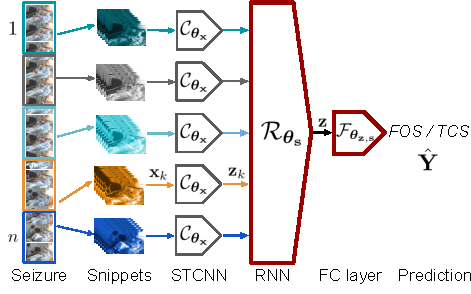
\includegraphics[width=0.8\textwidth]{diagram_gestures}
  \caption[Overview of the GESTURES architecture]{
    Our architecture: \acf{GESTURES}.
    We train only the models with thick red borders.
    FC stands for `fully-connected'.
  }
  \label{fig:gestures}
\end{figure}



\begin{figure}
  \centering
  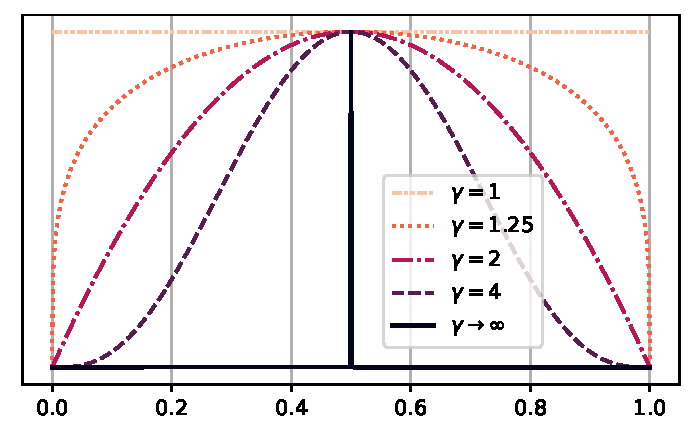
\includegraphics[width=0.7\textwidth]{beta}
  \caption[Probability distributions to sample snippets from video segments]{
    Probability distributions used to sample snippets from video segments.
  }
  \label{fig:betas}
\end{figure}



In this experiment, we compared the performance of three aggregation methods to perform seizure-level classification given a set of snippets, using
1) the mean,
2) an \ac{RNN} with 64 \ac{LSTM} units and
3) an \ac{RNN} with 64 \ac{BLSTM} units
to aggregate the $n$ feature vectors sampled from the video segments.
We used the dataset of feature vectors generated by \mbox{R(2+1)D-34 (8)} (\cref{sec:exp_feat}).
For the task of classifying \ac{FOS} and \ac{FBTCS}, the number of segments must be selected to ensure snippets after $t_G$, when generalizing semiologies begin, are sampled.
The theoretical minimum number of segments needed to sample snippets after $t_G$ is $n\st{min} = \lceil 1 / (1 - r\st{max}) \rceil $, where $r\st{max}$ is the largest possible ratio of non-generalizing to generalizing seizure durations (\cref{sec:dataset}).
We can estimate $r\st{max}$ from our dataset: $r\st{max} = \max ( r_1, \dots, r_{n\st{FBTCS}} ) = 0.93$, where $n\st{FBTCS}$ is the number of \acp{FBTCS}, which yields $n\st{min} = 15$ segments.
We evaluated model performance using $n \in \{2, 4, 8, 16\}$ segments per video and a sampling distribution using $\gamma \in \{ 1, 1.25, 2, 4, \infty \}$, corresponding to uniform, near semi-elliptic, parabolic, near Gaussian and Dirac's delta distributions, respectively.
For evaluation, we used $\gamma \rightarrow \infty$, i.e., only the central snippet of each segment.
We trained using mini-batches with sequences sampled from 64 videos, and an initial learning rate of $10 ^ {-2}$.
We used a weighted binary cross-entropy loss for training, where the weight for the \ac{FBTCS} class was the ratio of \acp{FOS} to \acp{FBTCS} in the training set.


\begin{figure}
  \centering
  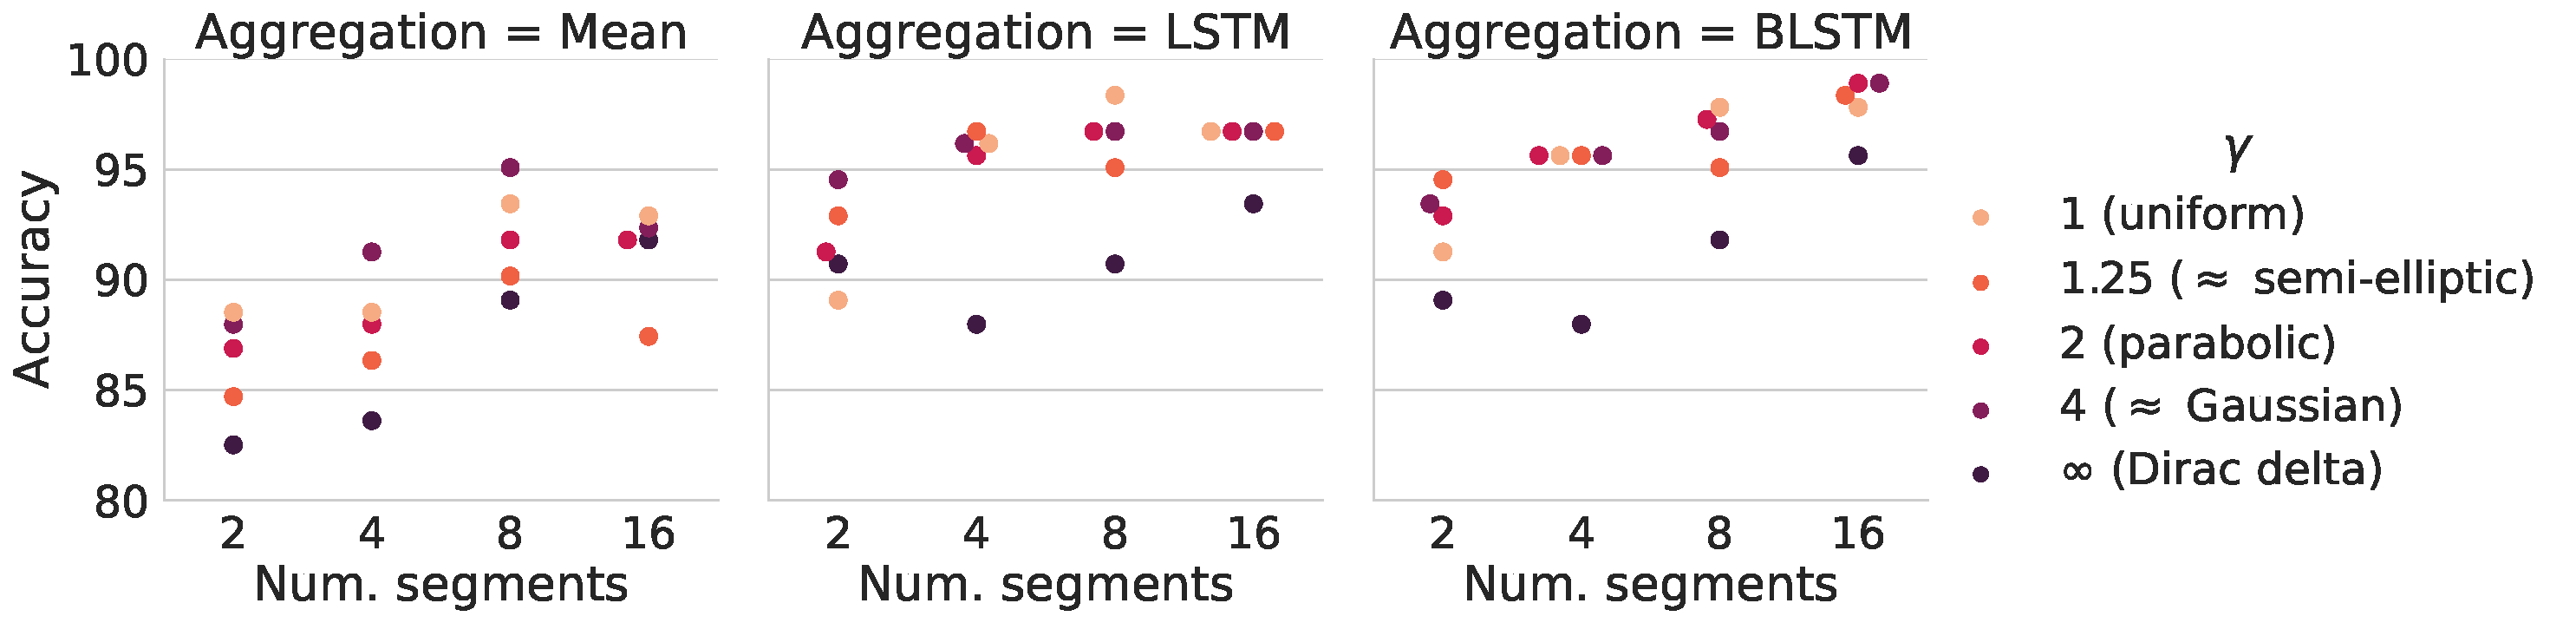
\includegraphics[width=\linewidth, trim=0 7 0 7, clip]{aggregation}
  \caption[Quantitative results for seizure-level classification]{
    Quantitative results for seizure-level classification.
    Marker brightness is proportional to the dispersion associated with the probability distribution used to sample snippets from the video segments (see \cref{fig:betas}).
  }
  \label{fig:aggregation}
\end{figure}

The highest accuracies were obtained using $n = 16$ segments, $\gamma \in \{ 2, 4 \}$ and the \ac{BLSTM} aggregator (\cref{fig:aggregation}).
The model with the highest accuracy (98.9\,\%) and $F_1$-score (98.7\,\%) yielded 77 true positives, 104 true negatives, 2 false positives and 0 false negatives, where \ac{FBTCS} is the positive class (\cref{sec:dataset}).
See the supplementary materials%
\fnurl{https://link.springer.com/chapter/10.1007/978-3-030-87240-3\_32\#Sec11}
for examples of videos classified correctly and incorrectly, with different levels of confidence.
